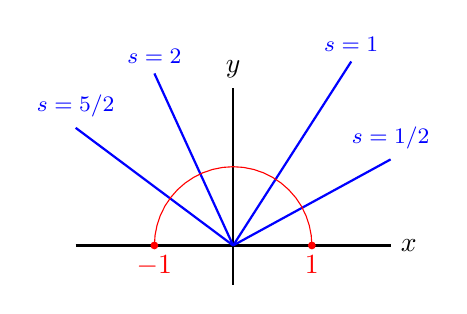
\begin{tikzpicture}
% Axis
\draw[thick] (-2,0)--(2,0) node[right]{$x$};
\draw[thick] (0,-0.5)--(0,2) node[above]{$y$};


\draw[thick, blue, domain=0:2, samples=25] plot(\x, {tan(1/2 r) *\x}) node [above]  {\footnotesize$s=1/2$};
\draw[thick, blue, domain=0:1.5, samples=25] plot(\x, {tan(1 r) *\x}) node [above]  {\footnotesize $s=1$};

% hack: set positive domain but draw -\x  so line is drawn from the origin to the end.
% This allows me to have the label at end of line instead of at the origin
\draw[thick, blue, domain=0:1, samples=25] plot(-\x, {tan(2 r) *-\x}) node[above]{\footnotesize$s=2$};
\draw[thick, blue, domain=0:2, samples=25] plot(-\x, {tan(5/2 r) *-\x}) node[above]{\footnotesize$s=5/2$};

\draw[red, domain=0:pi, samples=25] plot({cos(\x r)},{sin(\x r)});

\node[circle, fill, inner sep=-1pt, red] at (1,0) {};
\node[red,below] at (1,0) {$1$};

\node[circle, fill, inner sep=-1pt, red] at (-1,0) {};
\node[red,below] at (-1,0) {$-1$};

\end{tikzpicture}